\chapter{Measurement of the Jet Energy Resolution}
\label{chap:calibration}
% As seen in the anatomy section, particle interaction probabilities vary by a huge span. This necessitates a precise knowledge of the detector and resolutions of measurements. Things like Pile-up are a nuisance in this endeavor, also seen in the anatomy section, and needs to be properly accounted for.
The SM of particle physics makes predictions about the dynamics of quarks and gluons, yet these particles cannot be directly measured in the detector. Quarks and gluons hadronize to form hadrons which give rise to particle showers in the detector that are reconstructed as jets.
While \cref{chap:experiment} focused on the experimental setup to measure the signals deposited by hadrons, and \cref{chap:objects} described how the signals are reconstructed to form jets, this chapter gives an overview of the procedures that are used in the ATLAS experiment to calibrate the energy of measured jets. Only calibrated jets allow making meaningful comparisons between experimental measurements and theoretical predictions.
The experimentally measured jet is calibrated to the level of the particle jet. The calibration is experimentally challenging due to the rich environment at hadron colliders as well as the complicated nature of hadronic interactions in the detector. 

The intricacies of how the detector responds to incoming particle showers is first described in \cref{sec:detector-response}. \Cref{sec:jes-calibration} then describes the multi-stage procedure to calibrate the energy of PFlow jets and EMTopo jets to the scale of the particle jet, which is known as the \emph{jet energy scale}, or \emph{JES}.
It is also crucial to measure the \emph{jet energy resolution} (\emph{JER}), i.e., the precision with which the energy of a jet can be measured. \Cref{sec:jer} introduces how the JER can be parametrized and \cref{sec:jer-measurement} discusses how the ATLAS collaboration measures the JER in data from \RunTwo for PFlow jets and EMTopo jets, respectively. Particular focus is given on the measurement of the noise term of the JER, which arises due to both multiple pile-up interactions and electronic noise. \Cref{sec:jer-in-analysis} concludes this chapter with a description of how the measured JER is used in physics analyses.
%  and \cref{sec:improvements-jer-measurement} gives an outlook on potential future improvements for the JER measurements.

% is crucial in order to be able to correct the JER in MC such that it matches the one found in data.

% This chapter describes how jet calibration is facilitated at the ATLAS experiment. 
% how experimental jets relate to partons.
%As a jet is the closest signature of a quark or gluon that can be measured experimentally, special care needs to be taken in its definition to facilitate meaningful comparisons between experiment and theory.
%how MC simulations need to be calibrated to match the data.

%- Paper: paper presents the strategy used for the determination of the jet energy scale (JES) and resolution (JER) by the ATLAS experiment and its implementation as it pertains to the analysis of data from Run 2 of the LHC.

%- This publication focuses on calibrating jets reconstructed with the anti-𝑘𝑡 [1] algorithm with radius parameter 𝑅 = 0.4.


\section{Detector Response to Jets}
\label{sec:detector-response}
The response of the calorimeter to traversing particles is defined as the fraction of the particle's original energy that can be measured. The so-called \emph{jet response} is thus defined as the fraction of the energy of the particle-level jet that is deposited in the detector, which is dominated by the detector response to the showering particles that form the jet.
As mentioned in \cref{chap:objects}, the calorimeter cells are calibrated at the EM scale which means that electromagnetically interacting particles like photons and electrons are measured with a response of $e = 1$. The energy of hadrons cannot be fully captured and some fraction of the energy does not contribute to the calorimeter signals, resulting in a hadron response of $h < 1$. Various physics effects contribute to this behavior, that is known as non-compensating.
%The calorimeter is therefore referred to as being  and 
\begin{itemize}
    \item The showering hadrons transfer energy to atomic nuclei that may be broken up during the interaction or remain in excited states. Consequently, the binding energy that must be supplied to break up the nucleus is lost, and the energy in the excited states of the nuclei cannot be directly meausured. 
    % This energy is lost to compensate for the binding energy or in the excited states of the nuclei.
    % It’s not that the energy is lost to binding energy, it’s that the binding energy must be supplied to break up the nucleus.
    \item The showering hadrons may decay to non-interacting secondaries that escape the detector, for example in pion decays to a muon and a neutrino.
    \item The neutrons produced may only undergo elastic scattering and thus escape the detector.
\end{itemize}

The particle showers of a jet consist of both an EM component and a non-EM component. The EM component consists of EM sub-showers created by neutral pions that halt the hadronic decay chain by decaying into pairs of photons. The non-EM component includes all hadronic interactions.
The full jet response can be written as
\begin{equation}
    R(E) = e\fEM(E) + h\left(1 - \fEM(E)\right),
\end{equation}
where \fEM is the fraction of the jet that interacts electromagnetically. This fraction increases as the energy of the jet increases, because the number of interactions that produce neutral pions increases. The calorimeter response is therefore \emph{nonlinear} with increasing jet energy.

In addition to the aforementioned effects, that lead to a calorimeter that is non-compensating, other factors related to the experiment and reconstruction contribute to potential energy mismeasurements:
\begin{itemize}
    \item Non-functional (\emph{dead}) detector material.
    \item Inefficiencies in the topo-clustering algorithm.
    \item Energy deposits that are not taken into account due to the finite radius of the jet algorithm.
\end{itemize}

To determine the jet response in the experiment, the reconstructed jet \pT can be compared to the \pT of a well-calibrated or well-known \emph{reference object}. The reference object may constitute a well-measured physics object or system in data, as explained in \cref{subsec:insitu-calibration}, or a particle-level truth jet, that is accessible in MC simulation.
In the latter case, the truth jets are typically matched geometrically to the reconstructed jets by requiring them to be within a certain radius $\Delta R < R_{\text{matched}}$.
The so-called \emph{truth response} can then be defined as the ratio of the reconstructed jet \pT and the \pT of the matched truth jet,
\begin{equation}
    R_{\text{truth}} =  \frac{\pTreco}{\pTtruth},
\end{equation}
which is a useful quantity for calibrating the jet energy, which is explained in the next section.
%When the energy of the reconstructed jet is calibrated so that $\pTreco = \pTcalib$, the mean jet response is what is considered to be the jet energy scale (JES) and the width of the jet response constitutes the jet energy resolution (JER). The mean and width are determined from a Gaussian fit to the core of the response distribution, as shown in \cref{fig:truth-response}. 


\section{Jet Energy Corrections}
\label{sec:jes-calibration}
The goal of the jet energy correction is to correct for the non-linearity as well as the non-compensating nature of the calorimeter and to bring the average jet response to unity.
To this end, a calibration procedure is performed that consists of several stages. The procedure used to calibrate jets reconstructed with the \antikt algorithm with a radius parameter of $R = 0.4$ is illustrated in \cref{tab:jes-calibration} and is discussed in this section. At each stage, the jet is manipulated at the level of the fully reconstructed object which is represented as a massless four-vector. The energy of a jet can therefore be treated as equivalent to its momentum\footnote{The terms energy and momentum are thus often used interchangeably throughout this thesis}. More details on the calibration procedure can be found in \ccite{JETM-2018-05}.

\begin{table}
    \newImageResize{figures/calibration/jes-calibration.pdf}
    \caption[Summary of the different stages of the jet energy calibration.]{Summary of the different stages of the jet energy calibration. Each correction is applied to the four momentum of the jet. Taken from \ccite{JETM-2018-05}.}
    \label{tab:jes-calibration}
\end{table}

%The different steps use either MC simulation or data and are also applied to either MC or data, depending on the correction.
\subsection{Pile-up correction}
\label{subsec:pile-up-correction}
The reconstructed jet \pT is first corrected on an event-by-event basis to on average remove the energy coming from pile-up interactions. This is done in two steps: First, a correction is applied based on the \pT density of the pile-up, $\rho$, and the jet area, $A$. Then, a residual correction removes any residual \pT dependence on the number of primary vertices (to correct for in-time pile-up contributions), $N_\text{PV}$, and the average pile-up (to correct for out-of-time pile-up contributions), $\mu$.
The $\rho$ observable is estimated by the median \pT density of jets, calculated with jets reconstructed with the \kt algorithm\footnote{The \kt algorithm works analogously to the \antikt algorithm that is described in \cref{subsubsec:jet-algorithm}, but with different definitions of the distance measures:
    \begin{align*}
        d_{ij} & = \text{min}\left(p_{T_i}^2,p_{T_j}^2\right) \frac{\Delta R_{ij}^2}{R^2}, \\
        d_{iB} & = p_{T_i}^2.
        \label{eq:kt-distances}
    \end{align*}
    This causes low \pT inputs to be combined first, which is in contrast to the \antikt algorithm.
}
with radius parameter $R = 0.4$, positive-energy topo-clusters with \absetaST{2} as input, and no JVT requirement applied.
The jet area is determined using a procedure known as ghost association, where a large number of particles with four-vectors of infinitesimal magnitude are added to the event prior to the jet reconstruction and assigned to the jet with which they are clustered. The area of a jet is then calculated from the number of ghost particles associated to that jet.
The residual pile-up correction is based on a comparison with geometrically matched truth jets. The energy after all pile-up corrections, can be written as
\begin{equation}
    \label{eq:pTpusub}
    \pTPUsub = \pTreco - \rho \times A - \alpha \times \left( N_{\text{PV}} - 1\right) - \beta \times \mu,
\end{equation}
where $\alpha$ and $\beta$ are derived from fits to the \pT dependence on $N_{\text{PV}}$ and $\mu$, respectively.
The energy scale at this stage can be considered as the \emph{pile-up subtracted (energy) scale} and corresponds to the energy scale of the jet constituents, such that it is also referred to as the \emph{constituent scale}.

\subsection{MC-based correction to the particle level}
What follows is a purely MC-based calibration of the four-momentum of the jet, derived with simulated dijet events. The energy and direction of the reconstructed jets is corrected to on average match the ones of particle-level jets (truth jets).
To this end, truth jets are matched to reconstructed jets with $\pT > 7\,\GeV$, by requiring them to be within $\Delta R = 0.3$. In addition, no other activity is allowed in the vicinity of the jets, which is ensured by requiring the reconstructed (truth) jets to have no other reconstructed (truth) jet with $\pT > 7\,\GeV$ within $\Delta R = 0.6$ ($\Delta R = 1.0$).
The average jet response is then quantified by the mean of a Gaussian fit to the core of the $\EPUsub / \Etrue$ response distribution and derived in bins of \Etrue.
The jet calibration factor, also denoted \emph{JES factor} throughout this thesis, is taken as the inverse of the average energy response parametrized as a function of \EPUsub.
The exact procedure, referred to as \emph{numerical inversion}, is outlined in \ccite{PERF-2011-03}. The resulting average response is shown in \cref{fig:jes-calibration-jet-response} for different bins of \etadet. A similar procedure is used to correct biases in the reconstructed jet $\etadet$, which is detailed in \ccite{JETM-2018-05}.
Jets calibrated with the MC-based corrections are considered to be at the \emph{JES scale} and referred to as PFlow+JES jets or EM+JES jets in the following.

\begin{figure}[ht]
    \newImageResizeCustom{0.6}{figures/calibration/jes-calibration-jet-response.pdf}
    \caption[The average jet energy response.]{The average energy response as a function of the reconstructed jet energy, \Ereco. Taken from \ccite{JETM-2018-05}.}
    \label{fig:jes-calibration-jet-response}
\end{figure}

\subsection{Global sequential calibration}
The jet response is dependent on many factors related to the shower development in the calorimeter, such as the shower shape, the energy distribution and flavor of the showering particles, and the particle composition.
Differences are especially pronounced between quark-initiated and gluon-initiated jets.
% and leads to an increased JER.
The \emph{Global sequential calibration} (GSC) identifies six (five) observables for PFlow+JES jets (EM+JES jets) that model the mentioned effects. The jet truth response is then parametrized as a function of these observables and a numerical inversion procedure~\cite{PERF-2011-03} is performed for each of them in sequence.
The corrections of the GSC reduce the JER while leaving the mean energy response unchanged.
Jets that have the GSC applied are considered to be \emph{fully calibrated}, and their transverse momentum is labelled as \pTcalib. If not explicitly mentioned otherwise, the GSC is applied to jets that are referred to as PFlow+JES jets or EM+JES jets.
%- GSC scale (only affects resolution, not JES on average! (discuss?))
% From DANDOY: The GSC shifts the energy of individual jets while maintaining the mean energy response derived in the previous jet energy scale calibration.    

\subsection{\textbf{\emph{In~situ}} calibration}
\label{subsec:insitu-calibration}
A final calibration step accounts for the residual differences between the jet response in data and MC simulation, caused by imperfections in both the detector simulations and physics modelling. 
This calibration, known as \emph{\insitu} calibration, is derived by comparing the jet response in data and MC simulation, applying the following double ratio as the final correction factor:
\begin{equation}
    c = \frac{R_{\insitu}^{\text{data}}}{R_{\insitu}^{\text{MC}}} = \frac{ \langle  \pTcalibData / \pTrefData \rangle }{ \langle \pTcalibMC / \pTrefMC \rangle}.
\end{equation}
The average response, $R_{\insitu}$, is taken from the peak location found by fitting the distribution of the ratio of the \pT of a calibrated jet, \pTcalib, and a well-measured reference object, \pTref, with a Gaussian function.
The double ratio is parametrized as a function of \pTref and the final calibration obtained again with a numerical inversion procedure~\cite{PERF-2011-03}.
This correction is only applied to data.

% To this end, different event topologies are exploited that allow to measure the jet response with respect to a well-calibrated reference object. 
% The \insitu jet response is measured by comparing the \pT of a calibrated jet with a well-calibrated reference object. 
% The \insitu calibration consists of three methods.
The method currently used in the ATLAS collaboration is known as \emph{missing}-$E_{\rm T}$ \emph{projection fraction} (MPF)~\cite{PERF-2014-02} and uses the full hadronic recoil instead of a single jet as reference object. This makes the calibration robust against pile-up and jet reconstruction thresholds. The MPF calibration is performed using $Z$+jets and $\gamma+$jets with clean back-to-back topologies. 
The MPF method is complemented by the so-called \emph{multijet balance} method that allows calibrating high-\pT jets by comparing a system of well-calibrated low-\pT jets with a single high-\pT jet~\cite{PERF-2014-02}.
Both methods are statistically combined to provide a single smooth calibration across \pT. 
A third \insitu method, known as $\eta$ intercalibration, uses dijet events to correct the energy scale of forward ($0.8 \leq |\etadet| < 4.5$) jets to match those of central ($|\etadet| < 0.8$) jets using the \pT balance in dijet events~\cite{PERF-2014-02}.
%- Definition of truth jets reconstructed using stable final-state particles
%Truth jets are reconstructed using stable final-state particles and exclude muons, neutrinos, and particles from pile-up interactions. Truth jets are selected with the same 𝑝T > 7 GeV and |𝜂| < 4.5 thresholds as EMtopo and PFlow jets, and are geometrically matched to those jets using the angular distance Δ𝑅 with the requirement Δ𝑅 < 0.3.


\section{Parametrization of the Jet Energy Resolution}
\label{sec:jer}
Multiple physics and experimental effects contribute to a sizable JER. They scale differently with increasing energy of the jet. For calorimeter-based measurements, the effects can be grouped into three categories captured by three parameters: the \emph{noise term} ($N$), the \emph{stochastic term} ($S$), and the \emph{constant term} ($C$).
The relative JER can then be parametrized as
\begin{equation}
    \label{eq:jer-parametrisation}
    \frac{\sigma_{p_{\rm T}}}{p_{\rm T}} = \frac{N}{p_{\rm T}} \oplus \frac{S}{\sqrt{p_{\rm T}}} \oplus C,
\end{equation}
which is referred to as $N, S, C$ parametrization in the following.
This parametrization is based on both physics considerations as well as empirical evidence from studies of the JER in MC and data.
The following explains how the three different terms in \cref{eq:jer-parametrisation} can be inferred from physics considerations and what other effects must be considered.

\paragraph{The noise term} captures resolution effects from both energy deposits stemming from pile-up interactions and other noise such as electronic noise.
%The noise at cell level, as discussed in \cref{sec:calo-clustering}, cannot trivially be translated into a noise at jet level, due to several reconstruction threshold effects in the topo-clustering algorithm or the jet algorithm, as well as the non-trivial effect of the jet calibration on the JER.
These contributions are approximately independent of the jet energy and thus scale with $1 / \pT$ in the relative JER. A detailed discussion of the noise term and how it is measured in data are provided in \cref{sec:noise-term-meas}.

\paragraph{The stochastic term} is dominated by fluctuations related to the shower development in the calorimeter. Their impact on the relative JER scales with $1 / \sqrt{\pT}$ and they arise from various sources:
%The measurements of a calorimeter are subject to the following fluctuations:
\begin{itemize}
    %\setlength{\itemsep}{0.0em}
    % \item Shower fluctuations: fluctuations in the number of particles produced in the shower and in the EM fraction, \fEM.
    % \item Sampling fluctuations: fluctuations in the number of ionising particles crossing the active layers of the sampling calorimeter.
    % \item Photo-electron statistics: inefficiencies converting photons to electrical signals in the hadronic tile calorimeter.
    \item Fluctuations in the number of particles produced in the calorimeter shower and in the EM fraction, \fEM.
    \item Fluctuations in the number of ionising particles crossing the active layers of the sampling calorimeter.
    \item Fluctuations in the inefficiencies in converting photons to electrical signals in the hadronic tile calorimeter.
    \item Fluctuations of the amount of invisible energy from neutron production, binding energy losses, and nuclear excitation losses.
    \item Fluctuations in the number of heavily ionising particles, such as alpha particles.
\end{itemize}

\paragraph{The constant term} captures the effect of shower leakage, for example from energy depositions outside the jet radius, and detector inefficiencies. These effects scale with the energy of the jet and thus enter the relative JER as constant.

\paragraph{The physics considerations} outlined above only consider calorimeter-type measurements.
In the case of PFlow jets, additional effects come into play that can have non-trivial effects on the JER.
First it should be noted that some of the aforementioned effects are mitigated with PFlow jets because the calorimeter measurements are partially replaced by more precise track measurements from the ID. 
The impact on the JER from the tracks is expected to be small.
However, an additional contribution to the PFlow JER comes from the sizable amount of incorrectly subtracted energy in the PFlow algorithm.
This amount is captured in a term known as the \emph{confusion term} and fluctuations of it contribute to the JER. Details on the confusion term can be found in \ccite{PERF-2015-09}. It is unfeasible to derive from first principle how this effect scales with increasing energy of the jet and thus empirical studies need to be performed.

\paragraph{Other non-trivial effects} on the JER are introduced by the jet energy calibration, most notably the MC-based correction as well as the GSC.
Due to the non-linearity of the calorimeter, the applied JES factor is dependent on the jet \pT as shown in \cref{fig:jes-calibration-jet-response}. This means that also the energy fluctuations to which a jet is subjected are scaled by a larger factor at low \pT than at high \pT, which can spoil the parametrization shown in \cref{eq:jer-parametrisation}.
As the energy response varies most at low \pT, the noise term is especially affected by this.
Another complexity is introduced by the GSC, which reduces the JER across the entire \pT range in a way that cannot be derived from first principle. The effect is also important at low \pT and partially compensates for the effects introduced by the MC-based correction.

\paragraph{}
Despite the mentioned limitations, the JER parametrization shown in \cref{eq:jer-parametrisation} proves to be an adequate formula to represent the PFlow JER as well as the EMTopo JER.
% , which can be rested in MC simulated samples.
%The following describes how the JER can be measured in Monte Carlo and data.
%It is therefore used in the noise term measurement presented in \cref{sec:noise-term-meas}.
% \subsection{Estimation of the jet energy resolution in Monte Carlo simulation}
This can be tested in MC simulated dijet events, where the JER can be derived from the width of the truth response distribution divided by its mean,
\begin{equation}
    \label{eq:response-jer}
    \responsejer = \sigma \left( \frac{\pTcalib}{\pTtruth} \right) / \mu \left( \frac{\pTcalib}{\pTtruth} \right).
\end{equation}
The width and mean are taken from a Gaussian fit to the core of the distribution of the truth response. An example is shown in \cref{fig:truth-response}. The division by the mean in \cref{eq:response-jer} corrects for the residual non-closure of the jet calibration, which is sizable at low \pT\footnote{For jets at JES scale, the response diverges from unity by a maximum of about $5\%\,(3\%, 1\%)$ at $\pTtrue = 20\,(30, 50)\,\GeV$~\cite{JETM-2018-05}.}. 
The JER estimated with this method is referred to as \emph{Response JER} in the following and can only be derived in MC simulation.

\begin{figure}[t]
    \newImageResizeHalf{figures/calibration/truth-response.pdf}
    \caption[Distribution of the truth response for fully calibrated EM+JES jets.]{Distribution of the truth response for fully calibrated EM+JES jets within $\abseta < 0.7$ and $30 < \pTtruth < 30\,\GeV$, including a Gaussian fit to extract the mean and standard deviation.}
    \label{fig:truth-response}
\end{figure}

\Cref{fig:jer-parametrisation-a,fig:jer-parametrisation-c} show the Response JER as a function of \pTtruth for PFlow+JES jets and EM+JES jets, respectively, including the fitting function when using the parametrization shown in \cref{eq:jer-parametrisation}. It can be seen that the fitting function describes the trend of the JER very well for both jet collections.
% It can be seen, that the parametrisation is not optimal but is workable enough!
An illustration of the effect of the different terms as a function of the jet \pT is shown in \cref{fig:jer-parametrisation-b} and \cref{fig:jer-parametrisation-d}, respectively. The values of the three parameters, $N$, $S$, and $C$, correspond to the values found in the fits shown in \cref{fig:jer-parametrisation-a,fig:jer-parametrisation-c}.
It can be observed, that the impact of the noise term is considerably smaller for PFlow jets than for EMTopo jets.
The noise term for PFlow jets stays sub-dominant even at low \pT, while for EMTopo jets it becomes dominant at $\pT \lesssim 30\,\GeV$. The stochastic term for both jet collections is dominant across a large \pT range up to $\pT = 1000\,\GeV$, which is where the constant term becomes important.



\begin{figure}[t]
    \subfloat[] {
        \label{fig:jer-parametrisation-a}
        \newImageResizeCustom{0.46}{figures/calibration/NoiseTerm_withPileupResolution_EMPFlowJets_mc16d_00eta07_nominalFit.pdf}
    }
    \subfloat[] {
        \label{fig:jer-parametrisation-b}
        \newImageResizeCustom{0.46}{figures/calibration/Breakdown-of-JER-parameters-MC16dMCJERPFlow.pdf}
    } \\
    \subfloat[] {
        \label{fig:jer-parametrisation-c}
        \newImageResizeCustom{0.46}{figures/calibration/NoiseTerm_withPileupResolution_EMTopoJets_mc16d_00eta07_nominalFit.pdf}
    }
    \subfloat[] {
        \label{fig:jer-parametrisation-d}
        \newImageResizeCustom{0.46}{figures/calibration/Breakdown-of-JER-parameters-MC16dMCJER.pdf}
    }
    \caption[Response JER derived for fully calibrated jets.]{Response JER derived for fully calibrated (a) PFlow+JES jets and (c) EM+JES jets, including a fit with the parametrization shown in \cref{eq:jer-parametrisation}. A breakdown of the effect of the different terms in the fitting function is also shown for the results obtained with (b) PFlow+JES jets and (d) EM+JES jets.}
    \label{fig:jer-parametrisation}
\end{figure}

\FloatBarrier
\begin{figure}[t]
    \newImageResizeCustom{0.9}{figures/calibration/flow-chart-jer.pdf}
    \caption[Overview of the different stages involved in the JER measurement.]{Overview of the different stages involved in the jet energy resolution measurement. More details are provided in the text.}
    \label{fig:flow-chart-jer}
\end{figure}


\section{Measurement of the Jet Energy Resolution in Data}
\label{sec:jer-measurement}
For \RunTwo, the ATLAS collaboration uses a combination of two types of measurements to determine the JER in data. The measurements involve several steps that are summarized in the flow chart shown in \cref{fig:flow-chart-jer} and are explained in this section.
The first type of measurement is an \insitu method, similar to the \insitu jet energy calibration, and measures the JER over the full \pT range using dijet events, which is explained in \cref{subsec:dijet-balance}. The uncertainties of this method become sizable at low \pT which is why a second measurement is carried out that measures the noise term of the JER independently. This reduces the JER uncertainties at low \pT where the noise term is most important. \Cref{sec:noise-term-meas} describes the noise term measurement in great detail, as it was carried out by the author of this thesis.
Both measurements are finally combined in a statistical combination referred to as the \emph{JER combination}, which is described in \cref{subsec:jer-combination}.

\subsection{Jet energy resolution measurement using dijet events}
\label{subsec:dijet-balance}
%The dijet measurements derived in data by considering physics processes with a jet recoiling against a well-measured reference object. 
% The dijet measurement leverages the well-defined dijet systems in a method known as \emph{dijet balance}.
% In events that exhibit a clean $2 \rightarrow 2$ signature with two quarks in the initial- and final state, the transverse momenta of the jets are expected to balance each other, as they enter the detector \emph{back-to-back} in the $\eta$-$\phi$ plane. 
The dijet \insitu JER measurement exploits the clean $2 \rightarrow 2$ signature of dijet events, with two quarks in the initial state and two quarks in the final state. In well-defined systems like these, the transverse momenta of the calibrated jets are expected to balance each other, as they enter the detector \emph{back-to-back} in the $\eta$-$\phi$ plane. Any deviation from an exact balance can therefore be attributed to resolution effects, which is exploited in the method referred to as \emph{dijet balance} method. The resulting JER is referred to as \emph{Balance JER} in the following.
% and can be derived in data as well as in MC simulation.

The Balance JER is derived with selected dijet events that exhibit a clean back-to-back topology and contain at least one jet in a well-calibrated reference region ($0.2 \leq \absetadet \leq 0.7$).
An asymmetry is defined that compares the \pT of the well-measured jet in the reference region, \pTref, to the \pT of a \emph{probe jet}, for which the resolution is to be measured. The probe jet is allowed to be anywhere in the detector within \absetadetST{4.5}.
The JER is then extracted in different bins of \pTref and \absetadet using an iterative fitting procedure. For more details on how the asymmetry is defined, and the JER extracted, the interested reader is referred to \ccite{JETM-2018-05}.

The resulting Balance JER derived in dijet data and MC simulation is shown in \cref{fig:insitu-jer-dijet-only}.
As can be seen, the uncertainties become large at low \pT\footnote{Uncertainties on the dijet JER measurement mostly stem from the presence of additional radiation in the events which spoil the perfect back-to-back signature, biases due to the event selection, and uncertainties from the JES.}, and the dijet JER measurement is not able to probe the JER to values much lower than $\pT = 50\,\GeV$, which is the regime at which the noise term becomes important.\footnote{JER measurements that use different event topologies such as \Zjets events are able to provide more precise results also at lower \pT. For the JER measurement presented in this thesis, they were not included due to other complexities. A detailed discussion about this goes beyond the scope of this thesis. However, the independent derivation of the noise term as presented in \cref{sec:noise-term-meas} is still useful, even if other JER measurements are included.}
The noise term is therefore derived independently, as described below.

\FloatBarrier
\begin{figure}[ht]
    \newImageResizeHalf{figures/calibration/insitu-jer-dijet-only.pdf}
    \caption[Balance JER as a function of \pT.]{Balance JER as a function of \pT for PFlow+JES jets in the central region of the detector, measured in dijet events and MC simulation using Pythia8. Previously published in \ccite{JETM-2018-05}.}
    \label{fig:insitu-jer-dijet-only}
\end{figure}


\subsection{Measurement of the noise term}
\label{sec:noise-term-meas}
%The goal of the noise term measurement is to isolate and measure the impact of different noise contributions to the JER. 
%The noise present at calorimeter-cell level was discussed in \cref{sec:calo-clustering}. 

The goal of the noise term measurement is to quantify how much the fluctuations of noise contribute to the JER.
This requires to isolate the noise effects from other contributions to the JER which is challenging, especially when considering reconstruction threshold effects for example in the topo-clustering algorithm:
The energy of a calorimeter cell could be raised above the threshold to be included in the 420 topo-clustering algorithm (see \cref{sec:calo-clustering}) only because of an interplay of noise and other effects. The measurement of the noise term therefore relies on certain assumptions, that are mentioned in the relevant sections below.
%, which results in sizable systematic uncertainties on the measurement.
%In the JER combination, the noise term measurement still reduces the JER uncertainties at low \pT.

The full noise term of the JER can be decomposed into two terms,
\begin{equation}
    \Nfull = \sqrt{ \left(\Npileup \right) +  \left( \Nmuzero \right) },
\end{equation}
where \Npileup is the noise due to pile-up and \Nmuzero the residual noise that is present without any collision events.
The latter contribution is expected to be largely dominated by \emph{electronic noise} and is therefore denoted as electronic noise throughout this thesis.
Both terms are derived independently of each other,  using a multi-stage procedure as summarized on the left-hand side of \cref{fig:flow-chart-jer}.

The pile-up noise term is derived in \emph{zero-bias data} recorded in 2017. ``Zero-bias data'' are a collection of $pp$ collision events triggered on random bunch crossings, i.e., with zero bias on the selection of the events. Loosely described this dataset corresponds to events with ``pile-up only''. To validate the derivation in data a \emph{minimum-bias} MC sample with simulated dijet processes is used.
%``Minimum bias'' refers to the selection of events with the minimum possible requirements necessary to ensure that an inelastic collision occurred.
\footnote{Because simulated samples have to be actively produced and thus require at least some minimum requirements a zero-bias MC sample is not defined.}
% @From https://indico.desy.de/event/4176/contributions/69707/attachments/45757/56182/1.pdf
%‘Minimum bias’ is an experimentally defined term, referring to the selection of inelastic events
%with the minimum possible requirements necessary to ensure that an inelastic collision occurred.
%Minimum bias events can include both non-diffractive and diffractive processes, although the
%precise definition and relative contributions vary among experiments and analyses. Typically,
%minimum bias events are dominated by soft interactions, with low transverse momentum and
%low particle multiplicity.

% and is typically used to measure the pile-up activity in the detector that is present in any $pp$ collision event. 
The electronic noise is estimated in a dedicated MC sample that consists of simulated dijet events with no pile-up overlaid.

All dijet MC samples are simulated with \PYTHIA 8.230~\cite{Sjostrand:2007gs} using the {\textsc NNPDF2.3LO}~\cite{Ball:2012cx} set of PDFs and the A3~\cite{ATL-PHYS-PUB-2014-021} tune. 
%The difference between the samples used for the noise term measurement lies in the amount of pile-up that is overlaid and the event selection, that is, whether a hard scatter event must be present.


% In order to estimate systematic uncertainties on the noise term meausrement, two more datasets are used: A minimum bias MC sample and a dijet MC sample with pile-up corresponding to the 2017 data taking conditions.
%tab:calibration-data-mcsamples

% \subsection{Dataset and Monte Carlo samples}
% - Ingredients (put this in table):
% - zero-bias data sample with 2017 pile-up (for random cones)
% - zero-bias MC sample with 2017 pile-up -> for randon-cones non-closure uncertainty
% - standard dijet sample with 2017 pile-up (-> for JES scaling)
% - dijet sample without pile-up overlaid  (-> for electronic noise AND JES scaling)

% - Mininum bias sample: ATLAS will use the Minimum Bias Trigger Scintillators (MBTS)
% - described in page 136 of ATLAS experiment. BUT we don't use minbias data! We use zero bias data! and min bias MC!
% From a proceeding: https://cds.cern.ch/record/1639610/files/ATL-PHYS-PROC-2013-346.pdf
%We trigger the minimum bias events with dedicated scintillators called minimum bias trigger
%scintillators (MBTS) and we reconstruct the tracks with the inner detector only. The trigger
%scintillation counters are mounted on LAr endcap cryostats covering the radial dimension of
%the inner detector. 
% - Zero bias sample: A random trigger at Level-1 accepts all types of inelastic events zero bias.
% - Dijet sample
% - from random reddit thread: simulated minbias events would be events where something visible ends up inside the detector and zero bias would be where a bunch crossing happened but there was no requirement for something to be in the detector.

%% \begin{table}[t]
%     \centering
%     \begin{tabular}{l l l }
%         \toprule
%         Dataset / MC Sample & Pile-up condition             & Usage                                      \\
%         \midrule
%         Zero-bias data      & Recorded in 2017              & random cones                               \\
%         Mininum-bias MC     & corresponding to 2017 pile-up & random cones uncertainty                   \\
%         Dijet MC            & corresponding to 2017 pile-up & random cones uncertainty, JES scaling      \\
%         Dijet MC            & without pile-up               & noise at $\mu=0$, uncertainty, JES scaling \\
%         \bottomrule
%     \end{tabular}
%     \caption{
%         Samples considered in the JER noise term measurement.}
%     \label{tab:noise-term-samples}
% \end{table}

\begin{table}[b!]
    \centering
    {\small
        \begin{tabular}{ccccc}
            \toprule
            Process             & Generator                                                              & Tune                             & PDF set                                   & Cross section \\
                                & + fragmentation/hadronisation                                          &                                  &                                           & order         \\
            \midrule
            Dijet  & \PYTHIA 8.230~\cite{Sjostrand:2007gs}                                  & A14~\cite{ATL-PHYS-PUB-2014-021} & {\textsc NNPDF2.3LO}~\cite{Ball:2012cx}   & LO            \\
            Dijet no pile-up     & \PYTHIA 8.230 & A14                              & {\textsc NNPDF2.3LO}                      & LO            \\
            Dijet low pile-up     & \PYTHIA 8.230 & A14                              & {\textsc NNPDF2.3LO}                      & LO            \\
            \midrule
            Dijet minimum-bias     & \PYTHIA 8.186 & A14                              & {\textsc NNPDF2.3LO}                      & LO            \\
            \midrule
            \midrule
            Zero-bias data & & & & \\
            \bottomrule
        \end{tabular}
    }
    \caption{List of samples used for the noise term measurement. Information is given regarding the underlying-event tunes, the PDF parameter sets, and the perturbative QCD highest-order accuracy used for the normalization of the different samples. Abbreviations in the PDF names and cross sections are LO (leading order), NLO (next-to-leading order), and NNLO (next-to-next-to-leading order).}
    \label{tab:noise-term-samples}
\end{table}



\subsubsection{Estimation of the pile-up noise in zero-bias data}
\label{subsec:pile-up-noise}
The pile-up noise is measured by first determining the noise at the scale of the jet constituents, with a method known as \emph{random cones method}, and then extrapolating the constituent-scale noise to the JES scale. It is assumed that the pile-up noise is independent of the jet energy and the hard scatter, which is validated by a cross-check in MC.

% - As can be seen in the previous section, the measurement of the JER at low \pT has large uncertainties.
% - Therefore, an independent measurement of the noise term is important to reduce the uncertainties at low \pT.
%In a method referred to as \emph{random cones method}, the energy fluctuations expected due to pile-up are estimated.
%the energy found within two cones of radius \Rrandomcone is summed and compared to each other. This provides a measure of the fluctuations due to pile-up.


%the energy found within two cones of radius \Rrandomcone is summed and compared to each other. This provides a measure of the fluctuations due to pile-up.
\paragraph{Random cones method} The random cones method can be used to measure the energy fluctuations expected from pile-up within a cone of radius \Rrandomcone. The momentum distribution of particle flow objects of a single zero-bias data event is shown in \cref{fig:random-cones-balance-a}.
%The method is based on the assumption that the pile-up activity is spherically symmetric and independent of the hard scatter.
For each zero-bias event, the energies of all jet constituents (either PFlow objects or topo-clusters) found within two non-overlapping circular cones of radius \Rrandomcone are summed.
The random cones are placed at random $\phi$ and at random \abseta within a selected range.
The distribution of the difference of the energy within the cones, $\Delta \pTrandomcone = p_{\text{T}}^{\text{Rcone1}} - p_{\text{T}}^\text{Rcone2}$, when sampled over many events, provides a measure of the expected energy fluctuations to which a jet with $R = \Rrandomcone$ is subjected.
% The width of the resulting distribution of the \pTrandomcone difference, $\Delta \pTrandomcone$, when performing this for many events, 
The distribution is shown in \cref{fig:random-cones-balance-b} for random cones with radius $\Rrandomcone = 0.4$ within the central region of the detector (\absetaST{0.7}). The width of the distribution, labelled as $\sigmaRC$, is quantified by taking the \SI{68}{\percent} \emph{confidence interval} (CI), due to the non-Gaussian behavior\footnote{The non-Gaussian behavior is expected to be predominantly caused by topo-clustering threshold effects, that can lead to outliers in the $\Delta \pTrandomcone$ observable.}.
The noise term due to pile-up at constituent scale, \Npileupconstscale, is determined by
\begin{equation}
    \Npileupconstscale = \frac{\sigmaRC}{2\sqrt{2}},
\end{equation}
where \sigmaRC is divided by 2 to obtain the half-width and by $\sqrt{2}$ to obtain the fluctuations corresponding to just a single random cone~\cite{JETM-2018-05}.
The constituent-scale noise as measured in data and MC is shown in \cref{fig:const-scale-noise-results} as a function of \abseta and $\mu$.
The $\abseta$ bins are chosen such that they align with the granularity changes of the calorimeter (see \cref{subsec:calorimeter}). 
The difference between data and MC is observed to be significant ($\approx 20\,\%$). This discrepancy is confirmed in other studies of data recorded by the ATLAS experiment.\footnote{The author of this thesis contributed various studies to further understand this behavior. However, a clear cause of the discrepancy has not been identified so far. It is conjectured that the discrepancy is caused by a combination of effects related to the soft QCD model, the subsequent particle evolution, and the detector simulation.}
% \footnote{The results of the studies remain inconclusive how much of the remaining discrepancy is in the QCD model at the matrix element level, or how much is in the subsequent particle evolution & detector simulation, and it is likely a combination of effects.}
Since the effect is constant with pile-up and independent of the energy of the jet, the jet calibration can greatly mitigate the impact of this mismodelling.
%As \pTrandomcone corresponds to the sum of energies at the scale of the jet constituents, \Npileup corresponds to the noise at the scale of the constituents.

\begin{figure}[t]
    \subfloat[] {
        \newImageResizeCustom{0.46}{figures/calibration/zero-bias-event-deposits.pdf}
        \label{fig:random-cones-balance-a}
    }
    \subfloat[] {
        \newImageResizeCustom{0.46}{figures/calibration/random-cones-difference.pdf}
        \label{fig:random-cones-balance-b}
    }
    \caption[Sum of transverse momenta of particle flow objects and difference of the transverse momentum within two random cones.]{(a) Sum of transverse momentum of neutral and selected charged particle flow objects in an area of $\Delta \eta \times \Delta \phi = 0.2 \times 0.2$ from a zero-bias event from the 2017 dataset. (b) Difference of the transverse momentum within two random cones with radius $R = 0.4$ using neutral and selected charged particle flow objects for the zero-bias dataset recorded in 2017.
        Previously published in \ccite{SinglePublicPlotZeroBiasDeposits,PublicPlotsJER}.}
    \label{fig:random-cones-balance}
\end{figure}

\paragraph{Constituent scale noise} The constituent scale noise derived in the previous step needs to be scaled to the JES scale.
%, which requires the same calibration factor to be applied as in the MC-based jet calibration to the particle level (see \cref{sec:jes-calibration}).
%Due to technical reasons\footnote{The JES scale factor is not available in bins of \pTtruth which is required for the random cones method}, 
This scaling is obtained from an MC sample with simulated dijet events and 2017 pile-up conditions. The scale factors applied to \Npileupconstscale are determined by taking the mean of the distribution of the ratio $\pTcalib / \pTPUsub$ in bins of \pTtruth, where \pTcalib corresponds to the \pT of fully calibrated jets and \pTPUsub is defined as shown in \cref{eq:pTpusub}. Truth jets with $\pT > 7\,\GeV$ are matched geometrically ($\Delta R < 0.3$) to the reconstructed jets for this purpose, and no other reconstructed (truth) jet with $\pT > 7\,\GeV$ is allowed to be within $\Delta R < 0.6$ ($\Delta R < 1$) of the reconstructed (truth) jet.
The pile-up noise at JES scale divided by \pTtruth can be interpreted as the contribution to the relative JER from pile-up. This is presented in \cref{fig:pile-up-jer-vs-pt} for the central region of the detector.
The pile-up contribution is significantly lower for PFlow jets than EMTopo jets, reflecting the superior resolution of track-based measurement at low \pT compared to calorimeter-based measurements.
% Different considerations need to be made when quantifying the pile-up noise at JES scale, \Npileup. A straightforward approach is to fit $N/\pT$ to the distribution shown in \cref{fig:pile-up-jer-vs-pt}. 
%However, due to the \pT dependence of the JES scaling this does not provide the most accurate fit results. 
%Another option is to extract the pile-up noise in a given \pTtruth bin. 
The pile-up noise, \Npileup, is finally quantified by fitting $N/\pT$ to this distribution and extracting $N$. The results are shown in \cref{tab:prelim-jer-2018-noise-term-inputs}.


% TODO: Add discussion of binning. See Dag email from 2018-07-10
% Hi all,

% This is based on the discussion from today's JES/JER meeting.
% https://indico.cern.ch/event/734005/

% "Fine" |eta_det| bins based on response dependent calorimeter features (+less stats in forward region)
% 0 - 0.2 - 0.7 - 1.0 - 1.3 - 1.8 - 2.5 - 2.8 - 3.2 - 3.5 - 4.5

% Suggested "course" eta bins for JER combination + noise measurments
% 0-0.7
% 0.7-1.3
% 1.3-1.8
% 1.8-2.5
% 2.5-3.2
% 3.2-3.5 <= by far worst part of detector
% 3.5-4.5

% => 7 bins

% Some results from Tae Hyoun (Matthew) Park's JER measurements for jets with pT in 110-150 GeV
% Gray+black = data in-situ, green = MC truth
% Note how well the in-situ capture the truth JER (!)
% EM+JES:

% - Scaling of const scale to JES
% - Different options to do that
% - Fits N / pT 
% - Pile-up dependent noise term 
% - GSC complication

%This, however, assumes that the JES scaling is independent of the \pT of the jet, which is not the case due to the non-linearity of the calorimeter. The JES scale factor is about XX for jets with $\pT = 20\,\GeV$ and XX for jets with $\pT = 40\,\GeV$.
%This means that the pile-up noise is amplified more at lower \pT by multiplying the jet \pT with a larger JES factor. If this were to be considered, the noise term needs to be extended by a \pT-dependent term, $\Npileup = \NpileuppT$.

%- Studies of Response JER showed that the pT dependence of the noise term is mitigated by the GSC calibration. The GSC uses on global jet properties that cannot be defined on a constituent level as would be needed for the random cones method. 
%- Disadvantage of deriving something at constituent scale that is manipulated at the global level.


\paragraph{Cross-check in MC} A cross-check can be performed for the random cones method by comparing the Response JER extracted from two dijet MC samples, one with pile-up and one without pile-up. \Cref{fig:non-closure} shows a comparison of the Reponse JER extracted in the two samples, their quadratic difference, as well as the pile-up noise derived with the random cones method in MC simulation. 
The quadratic difference of the Response JER measurements in these samples is expected to be dominated by contributions from pile-up.
Comparing it to the noise extracted from MC simulation thus provides an estimate of the closure of the random cones method.
A non-closure uncertainty is quantified by comparing \Npileup as extracted from MC, to the parameter $N$ extracted from a fit of the functional form $N/\pT \oplus S/\sqrt{\pT}$ to the quadratic difference. The stochastic term is included here because it was found to be non-negligible in the quadratic difference, which is attributed mainly to the fact that the energy deposits from pile-up are also subject to stochastic fluctuations.

\paragraph{Uncertainty sources} Various sources of uncertainty need to be considered for the measurement of \Npileup. The dominant uncertainty comes from the method itself and is derived from the cross-check described above. Two more uncertainty sources are considered:
The first is related to the extraction of the constituent-scale noise and estimated by varying the definition of \sigmaRC: Instead of the 68\% CI, the 87\% CI divided by 1.5 is used as up variation and the 50\% CI multiplied 1.5 as down variation. This provides an estimate on the level of non-Gaussian behavior of the $\Delta \pTrandomcone$ observable. The second additional uncertainty source is related to the JES scaling and estimated by varying the JES scale factor. The mean of a Gaussian fit to $\pTcalib / \pTPUsub$ is therefore taken alternatively to the mean of the distribution itself. This uncertainty has only a small contribution to the overall uncertainty.

Additional uncertainties on \Npileup were tested and found to be negligible. These include uncertainties from varying the fit ranges used in the fits to the truth response distributions as well as JER fits, and the errors on the parameters from the fits themselves.

% \begin{itemize}
%     % \item \Npileup non-closure:
%     %       The noise extracted from the quadratic difference between the Response JER derived in a sample with and without pile-up is compared to the noise from the random cones method in MC simulation, as shown in \cref{fig:non-closure}. The difference is taken as an uncertainty.
%     \item Definition of \sigmaRC:
%           The definition of \sigmaRC is varied by using the 87\% CI divided by 1.5 and 50\% CI multiplied 1.5 instead of the 68\% CI. This provides an estimate on the level of non-Gaussian behavior of the $\Delta \pTrandomcone$ observable.
%     \item JES scale factor: the JES conversion factor is varied by using the mean of a Gaussian fit to $\pTcalib / \pTPUsub$ instead of its mean.
% \end{itemize}


\begin{figure}[t]
    \subfloat[] {
        \resizebox{0.5\textwidth}{!}{
            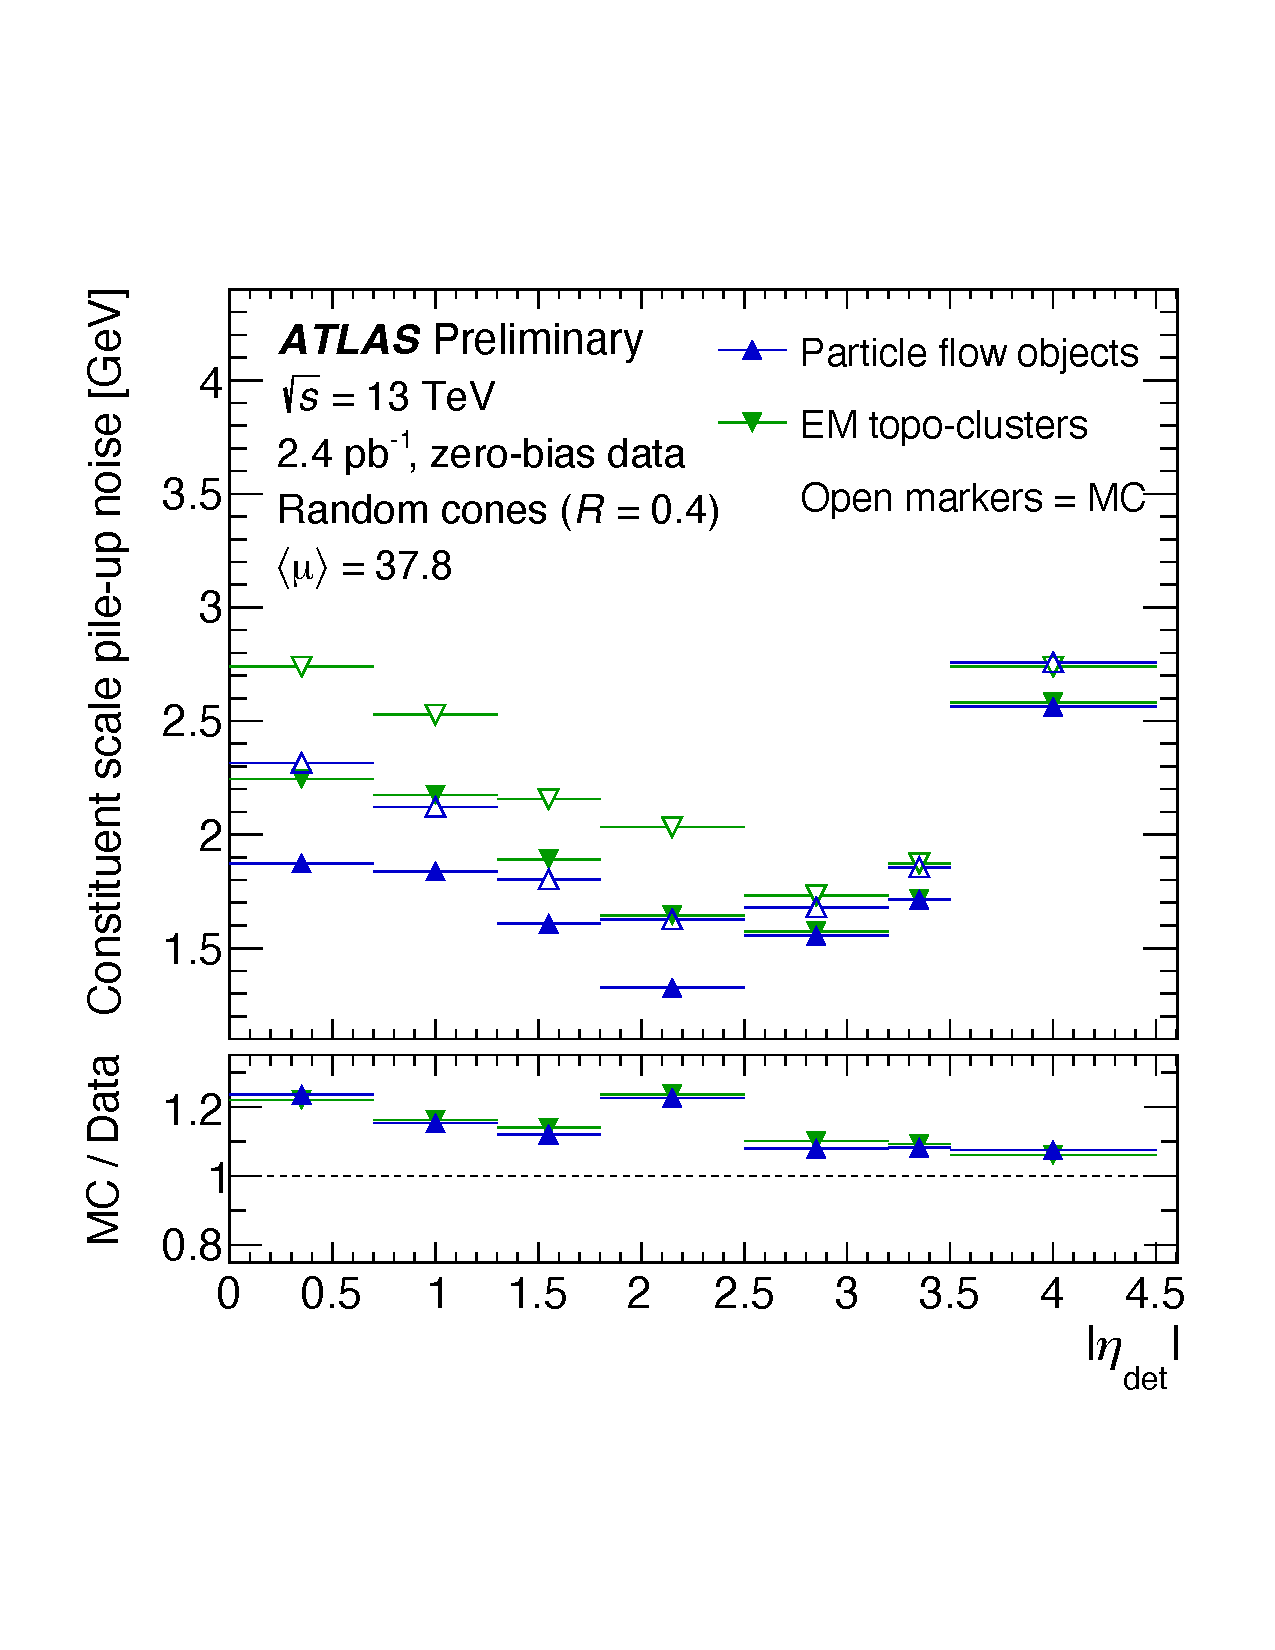
\includegraphics[trim=35 120 0 120]{figures/calibration/const-noise-vs-eta-new.pdf}
        }
    }
    \subfloat[] {
        \resizebox{0.5\textwidth}{!}{
            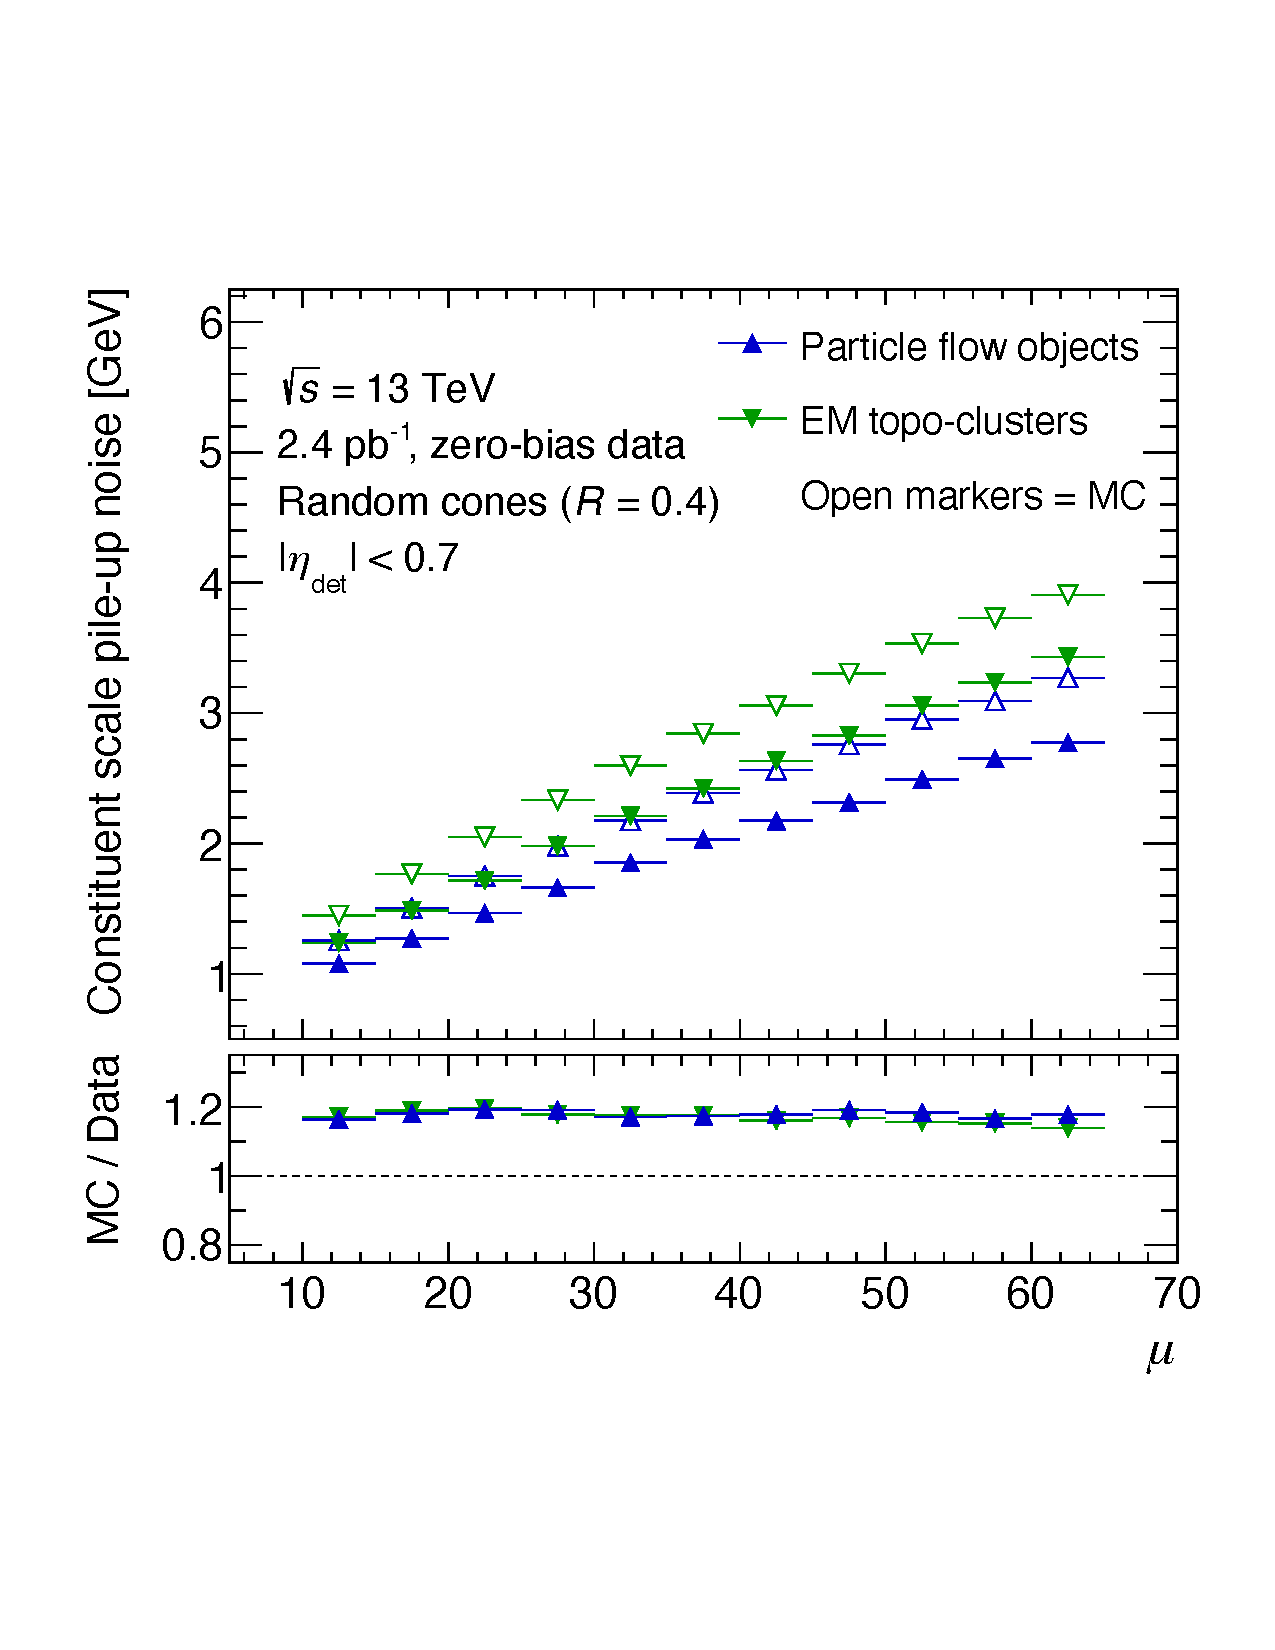
\includegraphics[trim=35 120 0 120]{figures/calibration/const-noise-vs-mu-new.pdf}
        }
    }
    \caption[Constituent-scale pile-up noise.]{Constituent-scale pile-up noise in \antikt $R=0.4$ jets (a) as a function of \absetadet and (b) as a function of $\mu$. Results are derived using the random cones method with either neutral and selected charged particle flow objects or topo-clusters at the electromagnetic scale as inputs. (a)
        Previously published in \ccite{PublicPlotsJER}.}
    \label{fig:const-scale-noise-results}
\end{figure}

% \begin{figure}[t]
%     \newImageResizeCustom{0.5}{figures/calibration/RandomCones_noise_over_eta_mc16d_MuDependenceStudy.pdf}
%     % from /Users/bj/offline_cernbox/AuthorshipQualification/Figures/180901/results/random-cones/RandomCones_noise_over_eta_mc16d_MuDependenceStudy.pdf
%     \caption{Constituent-scale pile-up noise in \antikt $R=0.4$ jets as a function of \absetadet for low pile-up ($\mu < 35$) and high pile-up ($\mu > 35$). Results are derived using the random cones method with either neutral and selected charged particle flow objects or topo-clusters at the electromagnetic scale as inputs.}
%     \label{fig:const-scale-noise-pileup-dependence}
% \end{figure}


\begin{figure}[t]
    \newImageResizeHalf{figures/calibration/pile-up-jer-vs-pt.pdf}
    \caption[The expected contribution to the JER from pile-up.]{The expected contribution to the jet energy resolution from pile-up extracted from 2017 data as a function of particle-jet \pT for \antikt jets with $R = 0.4$ in the central region of the detector $\absetadet < 0.7$. Previously published in \ccite{PublicPlotsJER}.}
    \label{fig:pile-up-jer-vs-pt}
\end{figure}



\begin{figure}[t]
    \newImageResizeCustom{0.5}{figures/calibration/random-cones-non-closure.pdf}
    \caption[Comparison between the pile-up noise term and the expectation from MC simulation.]{Comparison between the pile-up noise term \Npileup determined using the random cone method (black solid circles) and the expectation from MC simulation (orange squares) as extracted from the difference in quadrature of MC simulation with (red downward triangles) and without (blue upward triangles) pile-up. Results are shown at the PFlow+JES energy scale for jets in the central region of the detector $\absetadet < 0.7$. Previously published in \ccite{JETM-2018-05}.}
    \label{fig:non-closure}
\end{figure}



\subsubsection{Estimation of the electronic noise from Monte Carlo}
\label{subsec:electronic-noise-extraction}
%Certain assumptions therefore need to be made to measure the noise term:
% - noise at mu=0 separately measured from MC (with uncertainties)
%The electronic noise needs to be estimated separately from the pile-up noise.
The electronic noise is estimated separately from the pile-up noise, as the random cones method does not capture contributions to the JER from effects other than pile-up, mainly because of the effective noise reduction in the 420 topo-clustering algorithm.
A finite \Nmuzero is still expected in the presence of a hard scatter event.
For example, when considering a cell that contains signals that are just not enough to exceed the necessary energy thresholds for it to be included in the topo-clustering algorithm, additional electronic noise may lift the signals above the reconstruction threshold such that it is eventually considered in the jet reconstruction.
The amount of noise expected due to this is estimated by extracting the parameter $N$ from a fit with the $N, S, C$ parametrization to the Response JER derived in a dedicated MC sample that has no pile-up overlaid.
The results are shown in \cref{tab:prelim-jer-2018-noise-term-inputs}.

Two systematic uncertainties on the extraction of \Nmuzero are considered. The first captures the differences in the JER between data and MC simulation as found in the ATLAS JER measurement in 2010 without pile-up~\cite{PERF-2011-04} and is considered by applying a 20\% relative uncertainty on \Nmuzero. The second and larger uncertainty compares the nominal value of \Nmuzero to the one found using an alternative method. In this alternative method the dijet MC sample with pile-up is first split into several bins of pile-up ($\mu$) and the Response JER then derived in each of those bins. The parameter $N$ is extracted in each $\mu$ bin from a fit to the Response JER with the $N, S, C$ parametrization. To estimate \Nmuzero, the values of $N$ are extrapolated with both a linear and a quadratic fit to $\mu=0$. The maximum of the differences between the two extrapolated values and the nominal value of \Nmuzero is taken as a conservative systematic uncertainty.
Similar to the uncertainties on \Npileup, additional uncertainties on \Nmuzero due to fit range variations or errors from the fit parameters themselves were found to be negligible.


\subsubsection{Results}
% The uncertainties of the assumptions included in the method need to be propagated to the final results. To this end, a variety of uncertainty sources need to be considered by varying different quantities. 
% A variety of uncertainty sources need to be considered in the noise term measurement.
% The dominant uncertainty on \Npileup is the uncertainty of the method itself, derived from the closure test described in \cref{subsec:pile-up-noise}. The following is the complete list of uncertainties considered for the measurement of \Npileup:
% \begin{itemize}
%     \item \Npileup non-closure:
%           The noise extracted from the quadratic difference between the Response JER derived in a sample with and without pile-up is compared to the noise from the random cones method in MC simulation, as shown in \cref{fig:non-closure}. The difference is taken as an uncertainty.
%     \item Definition of \sigmaRC:
%           The definition of \sigmaRC is varied by using the 87\% CI divided by 1.5 and 50\% CI multiplied 1.5 instead of the 68\% CI. This provides an estimate on the level of non-Gaussian behavior of the $\Delta \pTrandomcone$ observable.
%     \item JES scale factor: the JES conversion factor is varied by using the mean of a Gaussian fit to $\pTcalib / \pTPUsub$ instead of its simple mean.
% \end{itemize}
% Systematics on the electronic noise, \Nmuzero, include the following:
% \begin{itemize}
%     \item MC vs data: ATLAS JER measurements in 2010 without pile-up~\cite{PERF-2011-04} showed that the noise term between data and MC is known to the level of 20\% uncertainty. This uncertainty is applied to \Nmuzero.
%           % \item Fit extraction uncertainty: the value of \Nmuzero is extracted from a fit to the Response JER with the $N, S, C$ parametrisation. This parametrisation is known to be sub-optimal. As well, the three parameters are highly correlated which adds additional uncertainty on the extracted value, $N$. 
%           % TODO: REVIEW THIS!!!!!!!!!!!!!!!!!!
%     \item Method uncertainty (fit instability): An alternative method to extract the noise at $\mu=0$ is performed. To this end, the dijet sample with pile-up is split into several bins of pile-up ($\mu$) and the Response JER is derived in each of those bins. The parameter $N$ is extracted in each bin from a fit with the $N, S, C$ parametrisation. The value of $N$ is then extrapolated with both a linear and a quadratic fit to $\mu=0$. The maximum of the differences between the two extrapolated values and the nominal value is taken as a systematic uncertainty.
% \end{itemize}

The measured values of the full noise term for both PFlow jets and EMTopo jets, as well as the breakdown into \Npileup and \Nmuzero, are presented in \cref{tab:prelim-jer-2018-noise-term-inputs}.
The uncertainties that were described in the sections above are propagated to \Nfull by varying them separately and observing the changes in \Nfull. Uncertainties that were estimated with only one variation are symmetrized.
The results vary considerably between different $\eta$ regions which is caused by the granularity changes of the calorimeter (see \cref{subsec:calorimeter}). For PFlow jets, it must also be taken into account that tracks can only be used within \absetaST{2.5}, which renders PFlow and EMTopo jets above $\abseta = 2.5$ very similar. This is also reflected in the results shown. While the noise term is considerably smaller for PFlow jets than for EMTopo jets within \absetaST{2.5}, the results become comparable at \absetaGT{2.5}. The uncertainties on the noise term are comparable, with small differences observed between different $\abseta$ regions.

The results of the noise term measurement for PFlow jets, including a breakdown of uncertainties, is illustrated in \cref{fig:noise-term-results-pflow}.
% From Paper: The systematic uncertainties enter the combined JER fit unsymmetrized in 𝜂 but are symmetrized during the statistical combination, and so the one-sided components are symmetrized in Figure 28 to illustrate their final contribution to the total uncertainty.
%\begin{table}[t]
    \centering
    \begin{tabular}{p{0.08\textwidth} | p{0.3\textwidth} | p{0.6\textwidth} }
        \toprule
                                  & Uncertainty                & Estimation                                                                     \\
        \midrule
        \multirow{2}{*}{\Npileup} & Non-closure                & Quadratic difference between MC JER derived in sample with and without pile-up \\
                                  & Const scale noise          & corresponding to 2017 pile-up                                                  \\
        \midrule
        \multirow{2}{*}{\Nmuzero} & Variations of fit function & varying fit function by                                                        \\
                                  & Fit error                  & Error from fit                                                                 \\
        \bottomrule
    \end{tabular}
    \caption{
        Uncertainties underlying the noise term measurement.}
    \label{tab:noise-term-uncertainties}
\end{table}

It can be seen, that the uncertainties on \Npileup, in particular the non-closure uncertainty, are dominant and become very large at \absetaGT{2.5}. This is where the detector granularity becomes significantly coarser and the calorimeter-cell noise thresholds have an increased impact on the JER. This causes the assumptions in the random cones method to become less valid, which is captured by a large non-closure uncertainty.
Also, the uncertainty from comparing \Nmuzero with the alternative estimate ($\mu=0$ fit instability) becomes sizable.


%that the contribution of pile-up to the JER is independent of the presence of a hard scatter becomes less valid. The closure uncertainty covers this effect.

%- electronic noise also more important at high eta
% - Add EMTopo jets comparison
% The noise term measurement was similarly performed for a different jet collection, known as \Rscan jets. 
% The procedure to derive the noise term is analog to what was presented here. The results are shown in \cref{app:noise-term-rscan}.

% \begin{table}[t]
    \centering
    \subfloat[]{
    \label{tab:improved-noise-term-inputs-a}
    \begin{tabular}{ l | c  c  c }
                             & \multicolumn{3}{|c}{MC16d, EMTopoJets}\tabularnewline
        \hline
                             & $N_{\text{pile-up}}$                                  & $N_{\mu = 0}$   & $N_{\text{full}}$\tabularnewline
        \hline
        $0.0 < |\eta| < 0.7$ & 3.86 $\pm$ 0.43                                       & 2.51 $\pm$ 0.52 & 4.61 $\pm$ 0.46\tabularnewline
        \hline
        $0.7 < |\eta| < 1.3$ & 4.16 $\pm$ 0.51                                       & 2.94 $\pm$ 0.62 & 5.09 $\pm$ 0.55\tabularnewline
        \hline
        $1.3 < |\eta| < 1.8$ & 3.83 $\pm$ 0.66                                       & 3.88 $\pm$ 0.84 & 5.46 $\pm$ 0.75\tabularnewline
        \hline
        $1.8 < |\eta| < 2.5$ & 2.69 $\pm$ 0.76                                       & 2.76 $\pm$ 0.57 & 3.85 $\pm$ 0.67\tabularnewline
        \hline
        $2.5 < |\eta| < 3.2$ & 2.52 $\pm$ 2.67                                       & 2.22 $\pm$ 0.45 & 3.36 $\pm$ 2.03\tabularnewline
        \hline
        $3.2 < |\eta| < 3.5$ & 3.41 $\pm$ 1.94                                       & 4.38 $\pm$ 1.04 & 5.55 $\pm$ 1.45\tabularnewline
        \hline
        $3.5 < |\eta| < 4.5$ & 3.68 $\pm$ 1.17                                       & 1.51 $\pm$ 0.44 & 3.98 $\pm$ 1.10
    \end{tabular}} \\
    
    \subfloat[] {
        \label{tab:improved-noise-term-inputs-b}

        \begin{tabular}{ l | c  c  c }
                                 & \multicolumn{3}{|c}{MC16d, EMPFlowJets}\tabularnewline
            \hline
                                 & $N_{\text{pile-up}}$                                   & $N_{\mu = 0}$   & $N_{\text{full}}$\tabularnewline
            \hline
            $0.0 < |\eta| < 0.7$ & 2.29 $\pm$ 0.54                                        & 0.00 $\pm$ 0.06 & 2.29 $\pm$ 0.54\tabularnewline
            \hline
            $0.7 < |\eta| < 1.3$ & 2.46 $\pm$ 0.78                                        & 0.00 $\pm$ 0.09 & 2.46 $\pm$ 0.78\tabularnewline
            \hline
            $1.3 < |\eta| < 1.8$ & 2.36 $\pm$ 1.13                                        & 0.85 $\pm$ 0.58 & 2.51 $\pm$ 1.08\tabularnewline
            \hline
            $1.8 < |\eta| < 2.5$ & 1.94 $\pm$ 1.55                                        & 1.26 $\pm$ 0.57 & 2.32 $\pm$ 1.34\tabularnewline
            \hline
            $2.5 < |\eta| < 3.2$ & 2.47 $\pm$ 2.88                                        & 1.96 $\pm$ 0.49 & 3.15 $\pm$ 2.28\tabularnewline
            \hline
            $3.2 < |\eta| < 3.5$ & 3.57 $\pm$ 2.33                                        & 3.16 $\pm$ 0.97 & 4.77 $\pm$ 1.86\tabularnewline
            \hline
            $3.5 < |\eta| < 4.5$ & 3.81 $\pm$ 1.25                                        & 0.00 $\pm$ 1.94 & 3.81 $\pm$ 1.25
        \end{tabular}
    }    
    \caption{
        Improved noise term inputs with a single \pT independent noise term.}
    \label{tab:improved-noise-term-inputs}
\end{table}
% \begin{table}[t]
    \centering
    \subfloat[]{
    \label{tab:pT-dependent-noise-term-inputs-a}
    \begin{tabular}{ l | c  c  c }
        & \multicolumn{3}{|c}{MC16d, EMTopoJets}\tabularnewline
       \hline
        & $N_{\text{pile-up}}$ & $N_{\mu = 0}$ & $N_{\text{full}}$\tabularnewline
       \hline
       $0.0 < |\eta| < 0.7$ & 4.75 $\pm$ 1.13 & 2.51 $\pm$ 0.52 & 5.38 $\pm$ 1.03\tabularnewline
       \hline
       $0.7 < |\eta| < 1.3$ & 5.42 $\pm$ 1.42 & 2.94 $\pm$ 0.62 & 6.17 $\pm$ 1.28\tabularnewline
       \hline
       $1.3 < |\eta| < 1.8$ & 5.17 $\pm$ 1.19 & 3.89 $\pm$ 0.84 & 6.47 $\pm$ 1.07\tabularnewline
       \hline
       $1.8 < |\eta| < 2.5$ & 3.31 $\pm$ 0.49 & 2.76 $\pm$ 0.57 & 4.31 $\pm$ 0.53\tabularnewline
       \hline
       $2.5 < |\eta| < 3.2$ & 3.03 $\pm$ 2.34 & 2.22 $\pm$ 0.45 & 3.76 $\pm$ 1.90\tabularnewline
       \hline
       $3.2 < |\eta| < 3.5$ & 4.10 $\pm$ 1.50 & 4.21 $\pm$ 0.90 & 5.88 $\pm$ 1.23\tabularnewline
       \hline
       $3.5 < |\eta| < 4.5$ & 4.18 $\pm$ 0.92 & 1.15 $\pm$ 1.20 & 4.33 $\pm$ 0.94
       \end{tabular}} \\
    \subfloat[] {
        \label{tab:pT-dependent-noise-term-inputs-b}
        \begin{tabular}{ l | c  c  c }
            & \multicolumn{3}{|c}{MC16d, EMPFlowJets}\tabularnewline
           \hline
            & $N_{\text{pile-up}}$ & $N_{\mu = 0}$ & $N_{\text{full}}$\tabularnewline
           \hline
           $0.0 < |\eta| < 0.7$ & 2.50 $\pm$ 0.40 & 0.00 $\pm$ 0.04 & 2.50 $\pm$ 0.40\tabularnewline
           \hline
           $0.7 < |\eta| < 1.3$ & 2.73 $\pm$ 0.59 & 0.00 $\pm$ 0.09 & 2.73 $\pm$ 0.59\tabularnewline
           \hline
           $1.3 < |\eta| < 1.8$ & 2.66 $\pm$ 0.93 & 0.92 $\pm$ 0.42 & 2.82 $\pm$ 0.89\tabularnewline
           \hline
           $1.8 < |\eta| < 2.5$ & 2.25 $\pm$ 1.31 & 1.26 $\pm$ 0.57 & 2.58 $\pm$ 1.17\tabularnewline
           \hline
           $2.5 < |\eta| < 3.2$ & 3.05 $\pm$ 2.47 & 1.98 $\pm$ 0.44 & 3.63 $\pm$ 2.08\tabularnewline
           \hline
           $3.2 < |\eta| < 3.5$ & 4.46 $\pm$ 1.68 & 2.65 $\pm$ 0.66 & 5.19 $\pm$ 1.48\tabularnewline
           \hline
           $3.5 < |\eta| < 4.5$ & 4.47 $\pm$ 0.92 & 0.00 $\pm$ 1.66 & 4.47 $\pm$ 0.92
           \end{tabular}
    }
    \caption{
        Noise term results extracted with a \pT dependent noise term and evaluated at $\pT = 30\,\GeV$.}
    \label{tab:pT-dependent-noise-term-inputs}
\end{table}

\begin{table}[t]
    \centering
    \subfloat[PFlow+JES jets] {
        \label{tab:prelim-jer-2018-noise-term-inputs-a}
        \begin{tabular}{ l | c  c  c }
            %                                    & \multicolumn{3}{|c}{MC16d, EMPFlowJets}\tabularnewline
            \toprule
                                    & $N_{\text{pile-up}}$ & $N_{\mu = 0}$    & $N_{\text{full}}$\tabularnewline
            \midrule
            $0.0 < |\etadet| < 0.7$ & 2.29 $\pm$ 0.38      & -0.00 $\pm$ 0.15 & 2.29 $\pm$ 0.38\tabularnewline
            \hline
            $0.7 < |\etadet| < 1.3$ & 2.42 $\pm$ 0.51      & 0.00 $\pm$ 0.21  & 2.42 $\pm$ 0.51\tabularnewline
            \hline
            $1.3 < |\etadet| < 1.8$ & 2.34 $\pm$ 1.22      & 0.61 $\pm$ 1.03  & 2.42 $\pm$ 1.21\tabularnewline
            \hline
            $1.8 < |\etadet| < 2.5$ & 2.01 $\pm$ 1.31      & 1.48 $\pm$ 1.51  & 2.49 $\pm$ 1.38\tabularnewline
            \hline
            $2.5 < |\etadet| < 3.2$ & 2.56 $\pm$ 2.99      & 2.02 $\pm$ 1.33  & 3.26 $\pm$ 2.49\tabularnewline
            \hline
            $3.2 < |\etadet| < 3.5$ & 3.64 $\pm$ 2.26      & 3.52 $\pm$ 1.59  & 5.07 $\pm$ 1.97\tabularnewline
            \hline
            $3.5 < |\etadet| < 4.5$ & 3.86 $\pm$ 1.27      & -0.00 $\pm$ 2.37 & 3.86 $\pm$ 1.27\tabularnewline
            \bottomrule
        \end{tabular}
    } \\
    \subfloat[EM+JES jets]{
        \label{tab:prelim-jer-2018-noise-term-inputs-b}
        \begin{tabular}{ l | c  c  c }
            \toprule
                                    & $N_{\text{pile-up}}$ & $N_{\mu = 0}$   & $N_{\text{full}}$\tabularnewline
            \midrule
            $0.0 < |\etadet| < 0.7$ & 3.86 $\pm$ 0.43      & 2.58 $\pm$ 1.07 & 4.64 $\pm$ 0.70\tabularnewline
            \hline
            $0.7 < |\etadet| < 1.3$ & 4.12 $\pm$ 0.63      & 2.98 $\pm$ 0.86 & 5.09 $\pm$ 0.72\tabularnewline
            \hline
            $1.3 < |\etadet| < 1.8$ & 3.76 $\pm$ 0.56      & 3.87 $\pm$ 0.96 & 5.40 $\pm$ 0.79\tabularnewline
            \hline
            $1.8 < |\etadet| < 2.5$ & 2.69 $\pm$ 0.41      & 2.85 $\pm$ 0.83 & 3.91 $\pm$ 0.66\tabularnewline
            \hline
            $2.5 < |\etadet| < 3.2$ & 2.55 $\pm$ 2.61      & 2.33 $\pm$ 0.71 & 3.46 $\pm$ 1.99\tabularnewline
            \hline
            $3.2 < |\etadet| < 3.5$ & 3.48 $\pm$ 1.93      & 4.70 $\pm$ 1.14 & 5.85 $\pm$ 1.47\tabularnewline
            \hline
            $3.5 < |\etadet| < 4.5$ & 3.76 $\pm$ 1.25      & 1.64 $\pm$ 1.67 & 4.10 $\pm$ 1.32\tabularnewline
            \bottomrule
        \end{tabular}}
    \caption[Results of the JER noise term measurement.]{Results of the noise term measurement for (a) PFlow+JES jets and (b) EM+JES jets, including a breakdown of the full noise term into the pile-up noise, \Npileup, and the electronic noise, \Nmuzero. The uncertainties correspond to the quadrature sum of the individual uncertainty sources described in the text. These results were used in the ATLAS JER combination for \RunTwo performed in 2018. }
    \label{tab:prelim-jer-2018-noise-term-inputs}
\end{table}

\begin{figure}
    \newImageResizeCustom{0.6}{figures/calibration/noise-term-results-pflow.pdf}
    \caption[Noise term of the JER and its uncertainties.]{Noise term of the jet energy resolution (JER) and its uncertainties as a function of \abseta. Previously published in \ccite{JETM-2018-05}.}
    \label{fig:noise-term-results-pflow}
\end{figure}


\subsection{Combined measurement of the jet energy resolution}
\label{subsec:jer-combination}
The JER combination is performed by fitting the dijet \insitu measurements (see \cref{subsec:dijet-balance}) with the functional form shown in \cref{eq:jer-parametrisation} with the noise term fixed to the values found in the noise term measurement (see \cref{sec:noise-term-meas}).

The resulting JER for PFlow jets is shown in \cref{fig:jer-combination-incl-noise-term-a}. The effect of the noise term is illustrated by displaying the nominally measured value $N / \pT$ including its uncertainties.
%The Balance JER taken from MC simulation can be compared to
The combined \insitu measurement shows significantly smaller uncertainties than the results of either the dijet balance method or the noise term measurement separately, which shows the benefit of the combination procedure.
%\TDnote{This is due to the fact that the combined measurement performs a simultaneous fit to all $\eta$ regions which leads to some uncertainties in the fit being constraint which is not reflected in the single measurements.}{Double-check this hypothesis.}

The final JER uncertainties are presented in \cref{fig:jer-combination-incl-noise-term-b}.
The uncertainties from the noise term measurement are propagated to the final results by varying the value of $N$ corresponding to each uncertainty source and repeating the fit. %The varied $N$ corresponds to the result that is obtained from the noise term measurement when the respective uncertainty is varied by one standard deviation.
The same procedure is applied to the uncertainties from the dijet \insitu measurement.
The uncertainties on the noise term have a sizable contribution at low \pT, but remain sub-dominant compared to the uncertainties from the dijet measurement.
% Mention correlation scheme? Therefore I have to explain the combination a bit more!
% An eigenvalue decomposition is performed to reduce the final number of nuisance parameters. This is done analogously to the eigenvalue decomposition used in the JES calibration for which a more detailed explanation can be found in \ccite{JETM-2018-05}.

A comparison of the JER between PFlow and EMTopo jets is shown in \cref{fig:jer-combination-results} for the central region of the detector.
At low \pT, PFlow jets outperform EMTopo jets and have a considerably lower JER as well as smaller JER uncertainties.
%This is also the case for other $\eta$ regions below $\etadet < 2.5$, which is shown in the figure.
%, as shown in \cref{fig:jer-combination-results-b}.
Above $\pT=100\,\GeV$ and beyond detector regions of $\etadet = 2.5$ (not shown), the JER of PFlow jets and EMTopo jets become similar, because the two jet collections themselves become very comparable, as fewer or no tracks are used as inputs to the \antikt algorithm in these regions of phase space. However, one difference remains between PFlow and EMTopo jets, which is the pile-up subtraction step in the jet calibration procedure (see \cref{subsec:pile-up-correction}). This explains the small differences that are still observed between the two jet collections.

\FloatBarrier
\begin{figure}[t]
    \subfloat[] {
        \newImageResizeCustom{0.46}{figures/calibration/combination-incl-noise-term-contribution.pdf}
        \label{fig:jer-combination-incl-noise-term-a}
    }
    \subfloat[] {
        \newImageResizeCustom{0.46}{figures/calibration/combination-unc-incl-noise-term-contribution.pdf}
        \label{fig:jer-combination-incl-noise-term-b}
    }
    \caption[The relative JER and the absolute uncertainty in the relative JER.]{(a) The relative jet energy resolution as a function of \pT for fully calibrated PFlow+JES jets. The error bars on points indicate the total uncertainties on the derivation of the relative resolution in dijet events, adding in quadrature statistical and systematic components. The expectation from Monte Carlo simulation is compared with the relative resolution as evaluated in data through the combination of the dijet balance and random cone techniques. (b) Absolute uncertainty on the relative jet energy resolution as a function of \pTjet. Uncertainties from the two \insitu measurements and from the data/MC simulation difference are shown separately. Figure and caption taken from \ccite{JETM-2018-05}.}
    \label{fig:jer-combination-incl-noise-term}
\end{figure}
\begin{figure}[t]
    \subfloat[] {
        \newImageResizeCustom{0.46}{figures/calibration/jer-combination-vs-pt.pdf}
        \label{fig:jer-combination-results-a}
    }
    \subfloat[] {
        \newImageResizeCustom{0.46}{figures/calibration/jer-unc-vs-pt.pdf}
        \label{fig:jer-combination-results-b}
    }
    \caption[The relative JER for fully calibrated jets.]{(a) The relative jet energy resolution and (b) the relative jet energy resolution systematic uncertainty for fully calibrated (blue curve) PFlow+JES jets and (green curve) EM+JES jets as a function of \pTjet. Taken from \ccite{JETM-2018-05}.}
    \label{fig:jer-combination-results}
\end{figure}

% \FloatBarrier
% \begin{figure}[t]
%     \subfloat[] {
%         \newImageResizeHalf{figures/calibration/jer-unc-vs-pt.pdf}
%     }
%     \subfloat[] {
%         \newImageResizeHalf{figures/calibration/jer-unc-vs-eta.pdf}
%     }
%     \caption{Fractional jet energy resolution systematic uncertainty summed across all components for \antikt $R = 0.4$ jets (a) as a function of jet \pTjet at $\eta = 0.2$ and (b) as a function of $\eta$ at $\pTjet = 30\,\GeV$. The total JER uncertainty is shown for both EM+JES and PFlow+JES jets. Taken from \ccite{JETM-2018-05}.}
%     \label{fig:jer-combination-uncertainties}
% \end{figure}

\section{Application of the Measured Jet Energy Resolution in Physics Analyses}
\label{sec:jer-in-analysis}
The measured JER is used to improve comparisons between MC simulations and data, both by both correcting the nominal JER of the MC simulations to on average match the one found in data and propagating systematic uncertainties of the JER measurements to the final event selection of physics analyses.
To this end, a procedure known as \emph{smearing} is applied in which the transverse momenta of the jets are randomly varied according to a Gaussian function with a certain width, labelled as $\sigma_{\text{smear}}$.

The nominal correction to the JER is only applied in regions of \pT and $\eta$ where the resolution in MC simulation is smaller than in data. In regions where the resolution in MC simulation is larger than in data, no nominal smearing is applied, but the full JER difference is taken as an additional systematic uncertainty.\footnote{Ideally, the JER in the MC simulation should be decreased (``unsmeared'') when it is larger than the one found in data. This, however, is technically challenging and computationally intensive, as it requires the comparison with truth information that is not always accessible in the MC simulation samples. Therefore, a conservative uncertainty is applied instead. This is planned to be revisited for future analyses.}

The systematic uncertainties are propagated by applying a Gaussian smearing with width
\begin{equation}
    \sigma_{\text{smear}} =  \left( \sigma_{\text{nom}} - |\sigma_{\text{variation}}|   \right)^2  - \sigma_{\text{nom}},
\end{equation}
where $\sigma_{\text{nom}}$ is the nominal value of the JER and $\sigma_{\text{variation}}$ corresponds to the JER that results when a certain systematic uncertainty is varied by one standard deviation.
% after one-standard-deviation variation of a certain systematic uncertainty.

In total 34 different uncertainty sources from the noise term and dijet measurements are considered in the JER combination across all $\abseta$ bins. To reduce the number of uncertainties that must be applied in physics analyses, an uncertainty reduction procedure is performed based on an eigenvalue decomposition. 
Different uncertainty reduction schemes can be used for this purpose, that result in a different number of uncertainties to be applied.
The scheme most widely adopted in \RunTwo ATLAS analyses comprises a set of 13 uncertainty sources.
Details of the uncertainty reduction procedure can be found in \ccite{JETM-2018-05}.

% From paper
% Also JER systematic uncertainties are propagated through physics analyses by smearing jets according to a Gaussian function with width 𝜎smear.


% \section{Future Improvements of the JER measurements}
% \label{sec:improvements-jer-measurement}
% - include Zjets balance
% - noise term measurement to split in mu bins

% - might not be relevant anymore -> PFlow jets

% - what to consider with higher pile-up in the future?

% - split in mu bins!!!
% - Factoring in GSC (hmm...I have to think about that again!)
% - Different JER parametrisation for PFlow

% - Maybe put that in an appendix.
